\documentclass[10 pt,usenames,dvipsnames, oneside]{article}
\usepackage{../../../modelo-ensino-medio}



\begin{document}

\begin{center}
  \begin{minipage}[l]{3cm}
\includegraphics[width=2cm]{logo}    
\end{minipage}\hfill
\begin{minipage}[r]{.8\textwidth}
 {\Large \scshape Atividade: Construa sua própria função periódica}  
\end{minipage}
\end{center}
\vspace{.2cm}

\ifdefined\prof
%Habilidades da BNCC
% \begin{objetivos}
% \item 
% \end{objetivos}

%Caixa do Para o Professor
\begin{sugestions}

%Orientações e sugestões
Caro professor, essa atividade é totalmente pessoal. É muito importante iniciar com o aluno determinando os eixos coordenados onde estarão para que assim ele possa situar a sua curva de maneira a correlacioná-la com alguma situação real e determinar período e amplitude. Uma ideia poderia ser o consumo de água de uma residência com 4 pessoas, suposto regular, durante o período de um dia em tempos de pandemia, em que os moradores não se ausentam de casa e realizam ali todas as refeições - tempo total: $20$ dias de observação, registros de consumo verificados a cada $6$ h, a partir das 6hrs da manhã, pensados em intervalos de madrugada ($0$ h-$6$ h), manhã ($6$ h-$12$ h), tarde ($12$ h-$18$ h), noite ($18$ h-$0$ h). Os registros diários de consumo seriam, por exemplo:
	\begin{itemize}[topsep=2pt]
	 \item madrugada - $20\ell$; 
	 \item manhã - $500\ell$; 
	 \item tarde - $60\ell$; 
	 \item noite - $300\ell$;
	 \end{itemize}
	 O gráfico poderia ser composto por uma linha poligonal, começando num ponto de ordenada $50$, depois passando por outro com ordenada $500$, depois por outro de ordenada $60$, outro de ordenada $300$ e em seguida um de ordenada $20$ e finalizando com outro ponto de ordenada $50$ (encerrando assim um ciclo do período da função). O gráfico da função periódica seria a repetição dessa poligonal. Teríamos então o gráfico sugerido a seguir, no qual o período é de $24$ h e a amplitude é $\frac{|20 - 500|}{2}=240$. Uma ideia interesse seria fazer uma análise crítica do contexto pensado com o gráfico produzido e pensar que modificações poderiam ser feitas no gráfico para que ele se adaptasse melhor ao contexto, numa perspectiva similar à realizada nas atividades do pêndulo realizadas no início do capítulo.
\end{sugestions}

\bigskip
\begin{center}
{\large \scshape Atividade}
\end{center}
\fi

Vamos fazer a nossa própria função periódica?

\begin{enumerate}
\item Usando a malha quadriculada proposta a seguir, defina, a origem, os eixos $Ox$ e $Oy$ e desenhe, usando até $6$ unidades horizontais da malha, uma curva que possa representar o gráfico de uma função, de modo que o ponto inicial da curva tenha mesma altura que o ponto final.
\item Agora, reproduza exatamente esse mesmo trecho por toda a largura da malha, do mesmo jeito como foi feito com a função dente de serra, construindo assim o gráfico de uma função periódica.
\item Qual o período e a amplitude da sua função periódica?
\item Compare o seu gráfico com o de seus colegas. Será que em pelo menos algum deles, você consegue imaginar um contexto real (climática, biológica, doméstica, tecnológica ou outras quaisquer) que ele poderia representar?

\end{enumerate}


\begin{figure}[H]
\centering


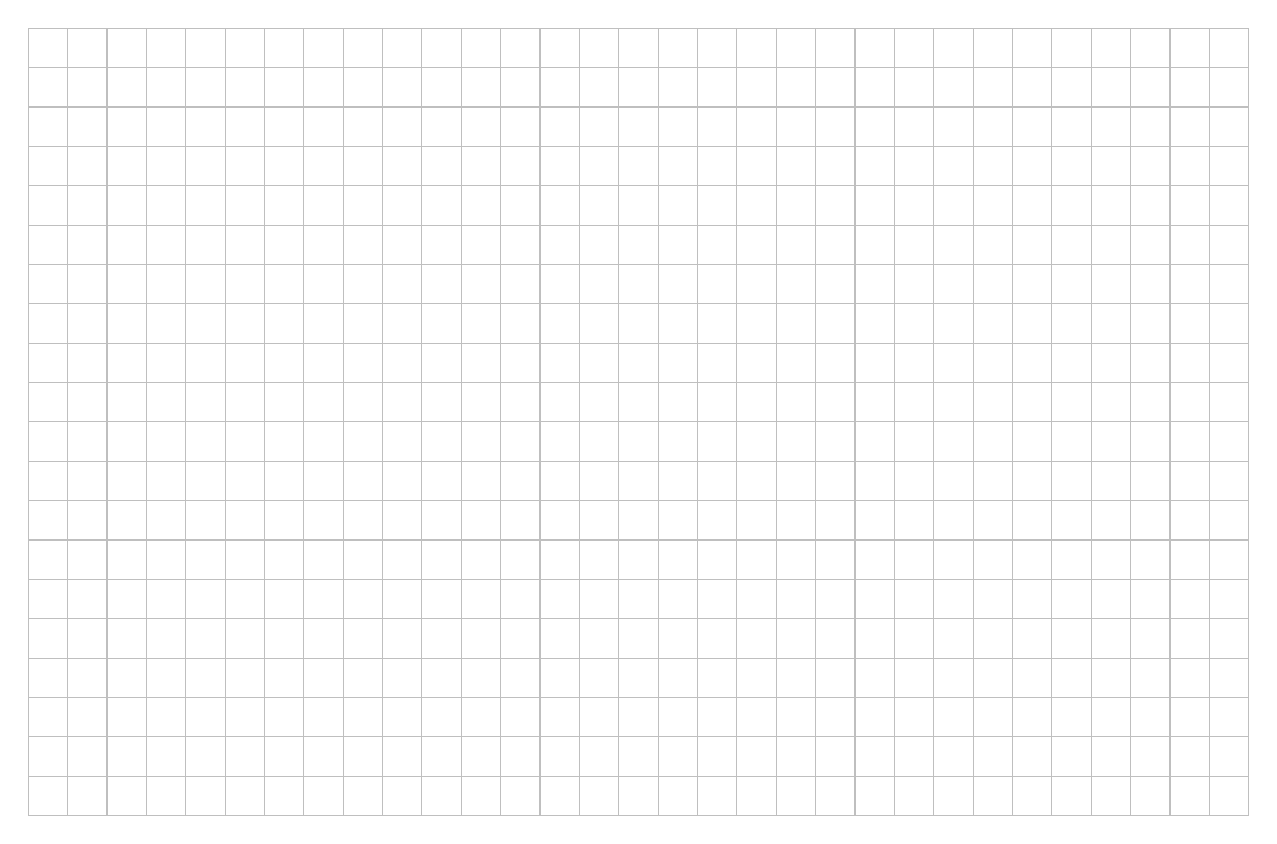
\begin{tikzpicture}
\draw [step=.5,gray!50] (-1.5,-5) grid (14,5);
\end{tikzpicture}

\end{figure}

% \ifdefined\prof
% \begin{solucao}

% \begin{enumerate}
% \item
% \end{enumerate}

% \end{solucao}
% \fi

\end{document}